%\documentclass[twocolumn,showpacs,preprintnumbers,amsmath,amssymb, floatfix]{revtex4}
\documentclass[aps,prb,preprint,preprintnumbers,amsmath,amssymb,floatfix,superscriptaddress]{revtex4}
%\documentclass[aps,prb,twocolumn,superscriptaddress,preprintnumbers,amsmath,amssymb,floatfix]{revtex4}

\usepackage{graphicx}
\usepackage{epstopdf}
\usepackage{ifthen}
\usepackage{dcolumn}
\usepackage{bm}
\usepackage{multirow}
\usepackage{booktabs}
\usepackage{amsbsy}
\usepackage{amsmath}
\usepackage{amssymb}
\usepackage{subfigure}
\usepackage{booktabs}

\graphicspath{
{/home/schuberm/Dropbox/git/plots.nogit/images}
}

%Definition of new commands
\newcommand{\f}[2]{\ensuremath{\frac{\displaystyle{#1}}{\displaystyle{#2}}}}
\newcommand{\lr}[1]{\langle{#1}\rangle}
\newcommand{\colv}[2] {\left(\begin{array}{c} #1 \\ #2 \end{array}\right)}
\renewcommand{\thefootnote}{\fnsymbol{footnote}}
\newcommand{\be} {\begin{eqnarray}}
\newcommand{\ee} {\end{eqnarray}}
%--------------------------------------------------------------------------
%EQ COMMANDS
%--------------------------------------------------------------------------
\newcommand{\two}{\mspace{-2.0mu}}
\newcommand{\four}{\mspace{-4.0mu}}
\newcommand{\plus}{\mspace{-4.5mu}+\mspace{-3.5mu}}
\newcommand{\minus}{\mspace{-4.5mu}-\mspace{-3.5mu}}
\newcommand{\pp}{'\mspace{-2.0mu}'}
\newcommand{\xlb}[4]{#1\ifthenelse{\equal{#2}{0}}{}{_{\alpha #2}}
\mspace{-2.0mu}\genfrac{(}{)}{0pt}{1}{\ifthenelse{\equal{#3}{0}}{0}{l #3}} 
{\ifthenelse{\equal{#4}{0}}{0}{b #4}}}

\newcommand{\xkv}[4]{#1\mspace{-5.0mu}\left(\mspace{-8.0mu}
\begin{smallmatrix}#2\four{}\four{}\mspace{-8.0mu}&\pmb{\kappa}#3\\&\nu 
#4\end{smallmatrix}\mspace{-5.0mu}\right)}

\newcommand{\evect}[6]{#1\mspace{-4.0mu}\left(\mspace{-8.0mu}
\begin{smallmatrix}#2\mspace{-8.0mu}&\pmb{\kappa} #3 &b #5\\&\nu #4 &
\alpha #6\end{smallmatrix}\mspace{-5.0mu}\right)}

\newcommand{\varmat}[8]{\mspace{-5.0mu}\left(\mspace{-8.0mu}
\begin{smallmatrix}\ifthenelse{\equal{#3}{0}}{\mspace{-8.0mu}&b_{#1}&b_{#2}
\\&\alpha_{#1}&\alpha_{#2}} {\ifthenelse{\equal{#7}{0}}{#1\mspace{-8.0mu}&
\pmb{\kappa}#2#3\mspace{-8.0mu}&\pmb{\kappa}#4#5\mspace{-8.0mu}&\pmb{\kappa}
#6\\&\nu#2&\nu#4&\nu#6} {#1\mspace{-8.0mu}&\pmb{\kappa}#2#3\mspace{-8.0mu}&
\pmb{\kappa}#4#5\mspace{-8.0mu}&\pmb{\kappa}#6#7\mspace{-8.0mu}&\pmb{\kappa}
#8\\&\nu#2&\nu#4&\nu#6&\nu#8}}\end{smallmatrix}\mspace{-5.0mu}\right)}

\newcommand{\EXP}[1]{\exp\mspace{-5.0mu}\left[#1\right]\mspace{-3.0mu}}

\newcommand{\tpp}[2]{\left(\mspace{-2.0mu}\xkv{\omega}{}{}{}#1\xkv{\omega}
{}{'}{'}#2\xkv{\omega}{}{\pp}{\pp}\mspace{-2.0mu}\right)}

%--------------------------------------------------------------------------
\newcommand{\SUM}[2]{\ifthenelse{\equal{#1}{0}}{\sum_{
\alpha_{#2},b_{#2},l_{#2}}^{3,n,N}} {\ifthenelse{\equal{#1}{1}}{\sum_{
\alpha_{#2},b_{#2}}^{3,n}}{\sum_{\pmb{\kappa}#2,\nu#2}^{N,3n}}}}

\newcommand{\SUMprime}[2]{\ifthenelse{\equal{#1}{0}}
{\sum_{\alpha_{#2},b_{#2},l_{#2}}^{3,n,N}} 
{\ifthenelse{\equal{#1}{1}}{\sum_{\alpha_{#2},b_{#2}}^{3,n}}
{\sum_{\pmb{\kappa}^{'}#2,\nu#2}^{N,3n}}}}

\newcommand{\SUMalpha}[2]{\ifthenelse{\equal{#1}{0}}
{\sum_{\alpha_{#2}}^{3}} {\ifthenelse{\equal{#1}{1}}
{\sum_{\alpha_{#2},b_{#2}}^{3,n}}{\sum_{\pmb{\kappa}#2,\nu#2}^{N,3n}}}}
%--------------------------------------------------------------------------
\newcommand{\SUMalphap}[2]{\ifthenelse{\equal{#1}{0}}
{\sum_{\alpha'_{#2}}^{3}} {\ifthenelse{\equal{#1}{1}}
{\sum_{\alpha'_{#2},b'_{#2}}^{3,n}}{\sum_{\pmb{\kappa}#2,\nu#2}^{N,3n}}}}

\newcommand{\SUMb}[2]{\ifthenelse{\equal{#1}{0}}{\sum_{b_{#2}}^{n}}
 {\ifthenelse{\equal{#1}{1}}{\sum_{\alpha_{#2},b_{#2}}^{3,n}}
{\sum_{\pmb{\kappa}#2,\nu#2}^{N,3n}}}}

\newcommand{\SUMbp}[2]{\ifthenelse{\equal{#1}{0}}{\sum_{b'_{#2}}^{n}}
 {\ifthenelse{\equal{#1}{1}}{\sum_{\alpha'_{#2},b'_{#2}}^{3,n}}
{\sum_{\pmb{\kappa}#2,\nu#2}^{N,3n}}}}

\newcommand{\SUMl}[2]{\ifthenelse{\equal{#1}{0}}{\sum_{l_{#2}}^{N}}
 {\ifthenelse{\equal{#1}{1}}{\sum_{\alpha_{#2},b_{#2}}^{3,n}}
{\sum_{\pmb{\kappa}#2,\nu#2}^{N,3n}}}}

\newcommand{\SUMlp}[2]{\ifthenelse{\equal{#1}{0}}{\sum_{l'_{#2}}^{N}}
 {\ifthenelse{\equal{#1}{1}}{\sum_{\alpha'_{#2},b'_{#2}}^{3,n}}
{\sum_{\pmb{\kappa}#2,\nu#2}^{N,3n}}}}

\newcommand{\abcdt}[5]{\mspace{-4.0mu}\left(\mspace{-8.0mu}
\begin{smallmatrix}&\ifthenelse{\equal{#1}{}}{a}{#1}&\ifthenelse
{\equal{#3}{}}{c}{#3}\\&\ifthenelse{\equal{#2}{}}{b}{#2}&\ifthenelse
{\equal{#4}{}}{d}{#4}\end{smallmatrix}\mspace{-2.0mu};\ifthenelse
{\equal{#5}{}}{t}{#5}\right)}

\newcommand{\abcd}[4]{\mspace{-4.0mu}\left(\mspace{-8.0mu}
\begin{smallmatrix}&\ifthenelse{\equal{#1}{}}{a}{#1}&\ifthenelse
{\equal{#3}{}}{c}{#3}\\&\ifthenelse{\equal{#2}{}}{b}{#2}&\ifthenelse
{\equal{#4}{}}{d}{#4}\end{smallmatrix}\mspace{-3.0mu}\right)}

\newcommand{\abt}[3]{\mspace{-4.0mu}\left(\mspace{-8.0mu}\begin
{smallmatrix}&\ifthenelse{\equal{#1}{}}{a}{#1} \\&\ifthenelse{
\equal{#2}{}}{b}{#2}\end{smallmatrix}\mspace{-2.0mu};
\ifthenelse{\equal{#3}{}}{t}{#3}\right)}

\newcommand{\ab}[2]{\mspace{-4.0mu}\left(\mspace{-8.0mu}
\begin{smallmatrix}&\ifthenelse{\equal{#1}{}}{a}{#1} \\&\ifthenelse
{\equal{#2}{}}{b}{#2}\end{smallmatrix}\mspace{-3.0mu}\right)}

\newcommand{\kvbat}{\mspace{-4.0mu}\left(\mspace{-8.0mu}
\begin{smallmatrix} &\pmb{\kappa} &b \\ &\nu &\alpha\end{smallmatrix}
\mspace{-2.0mu};t\right)}
%--------------------------------------------------------------------------
\newcommand{\kvbatp}{\mspace{-4.0mu}\left(\mspace{-8.0mu}
\begin{smallmatrix} &\pmb{\kappa} &b' \\ &\nu &\alpha'\end{smallmatrix}
\mspace{-2.0mu};t\right)}

\newcommand{\kvbaw}{\mspace{-4.0mu}\left(\mspace{-8.0mu}
\begin{smallmatrix} &\pmb{\kappa} &b \\ &\nu &\alpha\end{smallmatrix}
\mspace{-2.0mu};\omega\right)}

\newcommand{\kvbawp}{\mspace{-4.0mu}\left(\mspace{-8.0mu}
\begin{smallmatrix} &\pmb{\kappa} &b' \\ &\nu &\alpha'\end{smallmatrix}
\mspace{-2.0mu};\omega\right)}

\newcommand{\kvba}{\mspace{-4.0mu}\left(\mspace{-8.0mu}
\begin{smallmatrix} &\pmb{\kappa} &b \\ &\nu &\alpha\end{smallmatrix}
\mspace{-3.0mu}\right)}

\newcommand{\kvbap}{\mspace{-4.0mu}\left(\mspace{-8.0mu}
\begin{smallmatrix} &\pmb{\kappa}' &b \\ &\nu' &\alpha\end{smallmatrix}
\mspace{-3.0mu}\right)}
%--------------------------------------------------------------------------
\newcommand{\kpvba}{\mspace{-4.0mu}\left(\mspace{-8.0mu}
\begin{smallmatrix} &\pmb{\kappa}^{'} &b \\ &\nu &\alpha\end{smallmatrix}
\mspace{-3.0mu}\right)}

\newcommand{\kva}{\mspace{-4.0mu}\left(\mspace{-8.0mu}
\begin{smallmatrix} &\pmb{\kappa} \\ &\nu &\alpha\end{smallmatrix}
\mspace{-3.0mu}\right)}

\newcommand{\kvap}{\mspace{-4.0mu}\left(\mspace{-8.0mu}
\begin{smallmatrix} &\pmb{\kappa} \\ &\nu &\alpha'\end{smallmatrix}
\mspace{-3.0mu}\right)}

\newcommand{\kvb}{\mspace{-4.0mu}\left(\mspace{-8.0mu}
\begin{smallmatrix} &\pmb{\kappa} &b \\ &\nu \end{smallmatrix}
\mspace{-3.0mu}\right)}

\newcommand{\kvbp}{\mspace{-4.0mu}\left(\mspace{-8.0mu}
\begin{smallmatrix} &\pmb{\kappa} &b' \\ &\nu \end{smallmatrix}
\mspace{-3.0mu}\right)}

\newcommand{\kvt}{\mspace{-4.0mu}\left(\mspace{-8.0mu}
\begin{smallmatrix}&\pmb{\kappa} \\&\nu\end{smallmatrix}
\mspace{-2.0mu};t\right)}

\newcommand{\kvzero}{\mspace{-4.0mu}\left(\mspace{-8.0mu}
\begin{smallmatrix}&\pmb{\kappa} \\&\nu\end{smallmatrix}
\mspace{-2.0mu};0\right)}

\newcommand{\kpvt}{\mspace{-4.0mu}\left(\mspace{-8.0mu}
\begin{smallmatrix}&\pmb{\kappa}^{'} \\&\nu\end{smallmatrix}
\mspace{-2.0mu};t\right)}

\newcommand{\kvw}{\mspace{-4.0mu}\left(\mspace{-8.0mu}
\begin{smallmatrix}&\pmb{\kappa} \\&\nu\end{smallmatrix}
\mspace{-2.0mu};\omega\right)}

\newcommand{\kv}{\mspace{-4.0mu}\left(\mspace{-8.0mu}
\begin{smallmatrix}&\pmb{\kappa} \\&\nu\end{smallmatrix}
\mspace{-3.0mu}\right)}

\newcommand{\kvp}{\mspace{-4.0mu}\left(\mspace{-8.0mu}
\begin{smallmatrix}&\pmb{\kappa'} \\&\nu'\end{smallmatrix}
\mspace{-3.0mu}\right)}

\newcommand{\kw}{\mspace{-4.0mu}\left(\mspace{-8.0mu}
\begin{smallmatrix}&\pmb{\kappa} \\&\omega\end{smallmatrix}
\mspace{-3.0mu}\right)}

\newcommand{\kpvp}{\mspace{-4.0mu}\left(\mspace{-8.0mu}
\begin{smallmatrix}&\pmb{\kappa'} \\&\nu'\end{smallmatrix}
\mspace{-3.0mu}\right)}
%--------------------------------------------------------------------------
\newcommand{\lbt}{\mspace{-4.0mu}\left(\mspace{-8.0mu}
\begin{smallmatrix}&l \\&b\end{smallmatrix}\mspace{-2.0mu};t\right)}

\newcommand{\lbtp}{\mspace{-4.0mu}\left(\mspace{-8.0mu}
\begin{smallmatrix}&l' \\&b'\end{smallmatrix}\mspace{-2.0mu};t\right)}

\newcommand{\lt}{\mspace{-4.0mu}\left(\mspace{-8.0mu}
\begin{smallmatrix}&l\end{smallmatrix}\mspace{-2.0mu};t\right)}

\newcommand{\ltp}{\mspace{-4.0mu}\left(\mspace{-8.0mu}
\begin{smallmatrix}&l'\end{smallmatrix}\mspace{-2.0mu};t\right)}

\newcommand{\lb}{\mspace{-4.0mu}\left(\mspace{-8.0mu}
\begin{smallmatrix}&l \\&b\end{smallmatrix}\mspace{-3.0mu}\right)}

\newcommand{\lbp}{\mspace{-4.0mu}\left(\mspace{-8.0mu}
\begin{smallmatrix}&l' \\&b'\end{smallmatrix}\mspace{-3.0mu}\right)}
%--------------------------------------------------------------------------
%COMMANDS
%--------------------------------------------------------------------------
%--------------------------------------------------------------------------
\begin{document}

\title{Mean Free Paths of Phonons in Superlattices from Normal Mode Decomposition}
\author{Samuel C. Huberman}
\affiliation{Department of Mechanical \& Industrial Engineering, University of Toronto, 
Toronto, Ontario M5S 3G8, Canada}
\author{Jason M. Larkin}
\affiliation{Department of Mechanical Engineering\\Carnegie Mellon University\\Pittsburgh, PA 15213}
\author{Alan J. H. McGaughey}
%\email{mcgaughey@cmu.edu}
\affiliation{Department of Mechanical Engineering\\Carnegie Mellon University\\Pittsburgh, PA 15213}
\author{Cristina H. Amon}
\affiliation{Department of Mechanical Engineering\\Carnegie Mellon University\\Pittsburgh, PA 15213}
\affiliation{Department of Mechanical \& Industrial Engineering, University of Toronto, 
Toronto, Ontario M5S 3G8, Canada}

\date{\today}% It is always \today, today,
             %  but any date may be explicitly specified
\vspace{14mm}
  
\begin{abstract}

We use Normal Mode Decomposition to obtain phonon properties from quasi-harmonic lattice dynamics calculations and classical molecular dynamics simulations in unstrained Lennard-Jones Argon superlattices. The Relaxation-Time Approximation is used to predict cross-plane and in-plane thermal conductivity for a range of superlattice period lengths. We find that interspecies mixing reduces a phonon's mean free path and for short-period superlattices, the onset of mode localization is observed.

\end{abstract}
\maketitle

\section{Introduction}
Equilibrium \cite {PhysRevB.85.195302} and non-equilibrium \cite {PhysRevB.79.214307,PhysRevB.79.075316,PhysRevB.72.174302} studies have been performed on a variety of superlattices. Although these techniques make predictions about the trends of thermal conductivity, a mode by mode analysis is required to understand the effects of the secondary periodicity upon phonon properties. Prior models relied upon approximations of the specularity and diffusivity of the interfaces \cite {PhysRevB.57.14958} and lacked the computational power \cite {PhysRevB.70.081310}. Recent work \cite{Luckyanova16112012,doi:10.1021/nl202186y} used Density Functional Perturbation Theory. Unlike these works, where the phonon properties for short period superlattices is extended to larger period superlattices for computational reasons \cite{Luckyanova16112012} or interfacial mixing is neglected \cite{doi:10.1021/nl202186y}, we demonstrate the ability of Normal Mode Decomposition (NMD) to predict the phonon properties in unstrained superlattices with perfect and mixed interfaces without making such approximations.

\section{Modeling Framework}

Here we follow a modified version of the NMD procedure outlined by Thomas \cite {PhysRevB.81.081411}. Quasi-harmonic lattice dynamics (HLD) calculations, where the Taylor series of the lattice potential energy is truncated at the second-order terms and the equations of motion are recast in to an eigenvalue problem with $\pmb{D}(\pmb{\kappa})$ being the Hermitian harmonic force constant dynamical matrix \cite{dove_introduction_1993-3}
%%%
\begin{equation}\label{EQ:LD}
\omega^2_0 \kv {} \pmb{e} \kv {}=\pmb{D}(\pmb{\kappa}) \pmb{e} \kv{},
\end{equation}
are performed to extract eigenvectors, $\pmb{e} \kv{}$, frequencies $\omega^2_0 \kv {}$ and group velocities, $\pmb{v}_{g}$
\begin{equation}\label{EQ:VG}
\pmb{v}_{g}\kv{}=\frac{\partial \omega}{\partial \pmb{\kappa}}.
\end{equation}
%%%
The allowed wavevectors, $\pmb{\kappa}$, are selected in accordance with the number of repetitions of the unit cell used in the classical molecular dynamics (MD) simulations 
%%%
\begin{equation}\label{EQ:NMD:allowdkpt}
\pmb{\kappa} = \sum_{\alpha} \pmb{b}_{\alpha} \frac{n_{\alpha}}{N_{\alpha}},
\end{equation}
%%%
where $\pmb{b}_\alpha$ are the reciprocal lattice vectors and $ \frac{N_\alpha}{2} < n_\alpha \le \frac {N_\alpha}{2}$, where n are integers and N are now constant even integers. The wavevectors are taken to be in the first Brillouin zone. The eigenvectors are used to construct a basis upon which the velocities are projected to obtain the time series of the normal mode coordinate 
%%%
\begin{equation}\label{EQ:NMD:qdot}
\begin{split}
\dot{q}\kvt{}{}{}=&\SUM{0}{}\sqrt{\frac{m_b}{N}}\dot{u}_{\alpha}\lbt e^*\kvba\EXP{i\pmb{\kappa}\cdot\mathbf{r}_0\ab{l}{0}},
\end{split}
\end{equation}
%%%
where $\dot{u}_{\alpha}\lbt$ is the component of velocity of atom $b$ in the $l$ th unit cell in the $\alpha$ direction and $e^*\kvba$ denotes the complex conjugate of the $\alpha$ component for atom $b$ of the $\kv$ eigenvector. By taking the Fourier transform of the autocorrelation of the normal mode coordinate, the spectral energy density (SED) is resolved \cite{dove_introduction_1993-3}
%%%
\begin{equation}\label{EQ:NMD:SED}
\begin{split}
T\kvw=&\lim_{\tau_0\rightarrow\infty}\frac{1}{2\tau_0}\left|\frac{1}{\sqrt{2\pi}}\int_{0}^{\tau_0}\dot{q}\kvt\exp(-i\omega t)dt\right|^2.\\
\end{split}
\end{equation}
%%% 
In accordance with anharmonic theory, the SED can be approximated to be a  Lorentzian of the form for cases where $\Gamma\kv \ll \omega_0\kv$ \cite{maradudin_scattering_1962}
%%%
\begin{equation}\label{EQ:NMD:LOR}
\begin{split}
T\kvw\approx&C_0\kv\frac{\Gamma\kv/\pi}{[\omega_0\kv-\omega]^2+\Gamma^2\kv},
\end{split}
\end{equation}
%%%
and thus fitting Equation~\ref{EQ:NMD:LOR} to Equation~\ref{EQ:NMD:SED} yields the phonon lifetime
%%%
\begin{equation}\label{EQ:lifetime}
\begin{split}
\tau\kv=&\frac{1}{2\Gamma\kv}\\
	=&\frac{1}{\Delta \omega \kv {}}.
\end{split}
\end{equation}
%%%
This spectral width corresponds to all possibles mechanisms of phonon interaction since no \textit{a priori} assumptions about such interactions were involved in its determination (and the effect of the secondary periodicity is captured by using the modified phonon dispersion). Thus all phonon-phonon scattering probabilities are enveloped into this single quantity. For bulk classical systems, where the only mechanisms for scattering are phonon-phonon processes, the MFP would be calculated as
%%%
\begin{equation}\label{EQ:M:phonon_mfp}
\begin{split}
\Lambda\kv &= |\pmb{v}_{g}\kv {}| \tau\kv.
\end{split}
\end{equation}
%%%
However, since $\tau\kv$ captures all involved scattering mechanisms that occur in a superlattice (and thus all phase randomizing mechanisms), this length can be referred to the effective mean free path.
Under the Boltzmann Transport Equation single mode relaxation time approximation \cite{ziman_electrons_2001}, the thermal conductivity in the $i$th direction is the summation across all contributing modes
%%%
\begin{equation}\label{EQ:M:conductivity}
\begin{split}
k_{vib,\mathbf{i}}=&\sum_{\pmb{\kappa}} \sum_\nu c_{ph}\kv 
\pmb{v}^{2}_{g,\mathbf{i}}\kv \tau\kv
\end{split}
\end{equation}
%%%
NMD calculations were conducted for a range of period lengths for Lennard-Jones Argon superlattices with a mass ratio ($m_A/m_B$) of 3 at a temperature of 20 K. MD was conducted using the LAMMPS package \cite{LAMMPS}. The LJ potential was set to be the same for all possible pairwise interactions with $\epsilon= 1.67E-21$ J and $\sigma= 3.4E-10$ m. The time step for MD was set to 4.285 fs. Atomic velocities were collected over a total span of $2^{20}$ time steps; the Fourier transform sampling window was set to $2^{16}$ time steps and the lag between velocities samples was $2^5$. This was sufficient to capture the highest frequency modes. Five independent MD simulations with different initial conditions were run and the SED was averaged over all seeds and Fourier transform sampling window. Further averaging was conducted by observing the symmetry of the Brillouin zone. Since the Brillouin zone is a rectangular prism, an arbitrary $\pmb{\kappa}$ is equivalent to 11 wavevectors in the Brillouin zone. HLD was conducted using GULP \cite{GULP}. Group velocities were calculated using finite differencing. A superlattice unit cell consisted of N conventional FCC unit cells of $m_A$ and N unit cells of $m_B$ along the cross-plane direction, thus a 2x2 superlattices refers to a superlattice period of 2 monolayers of $m_A$ and 2 monolayers of $m_B$. Size effects were accounted for by performing a convergence study. It was found predictions in both cross-plane and in-plane thermal conductivities varied negligibly for systems with more than $N_x=8$ superlattice UCs along the cross-plane and $N_y=N_z=6$ UCs along the in-plane.

Following the approach put forward by Landry \cite{PhysRevB.79.075316}, interspecies interfacial mixing was controlled by selecting the individual adjacent monolayers to an interface in the MD computational cell and flipping the masses of randomly selected atoms until the desired concentrations were reached. For example, a mixing of 80/20 refers an original/foreign blend in an adjacent monolayer. It was assumed that the eigenvectors remained unchanged by introduction of mixing which is presumed to be valid under small perturbations from the original system. The effects of this assumption can be observed in Figure~\ref{fig:sed}, where for the majority of the modes, the peaks remain well-defined, but some become noticeably perturbed. However, fitting a Lorentzian was deemed suitable as the coefficient of determination value for the most effected modes was about 0.9. The consequences of making such an assumption is reviewed in the following section. No lattice strain was permitted as the effects have been studied elsewhere \cite{PhysRevB.72.174302}.

The specific heat is set to be $\frac{k_B}{V}$ per mode, where V is the system volume of the MD computational domain, because the systems considered here are classical and obey Maxwell-Boltzmann statistics. As temperature increases, anharmonicity of the potential energy decreases the specific heat from $\frac{k_B}{V}$. However, the effect is small for these superlattices at 20 K.

\section{Results}
%%%
\renewcommand{\topfraction}{0.7}
\begin{figure*}[ht!]
\begin{center}
\scalebox{1}{ \includegraphics{/home/schuberm/Dropbox/git/plots.nogit/images/4p_dispersion.eps}}
\renewcommand{\figure}{Fig.}
\caption{Dispersion of a 4x4 superlattice for modes normal to the interfaces. Red squares represent select modes for k=[1,0,0].}
\label{fig:dispersion}
\end{center}
\end{figure*}
%%%
Sample peaks are shown in Figure~\ref{fig:sed}. Note that while the peaks appear to be Lorentzian centered about single frequency, there are minor signatures at other frequencies. Such peaks are attributed to the approximation that the normal mode of the harmonic system is equivalent to the normal mode of the anharmonic system.
%%%
\begin{figure}[!h]
\begin{center}
\scalebox{1}{ 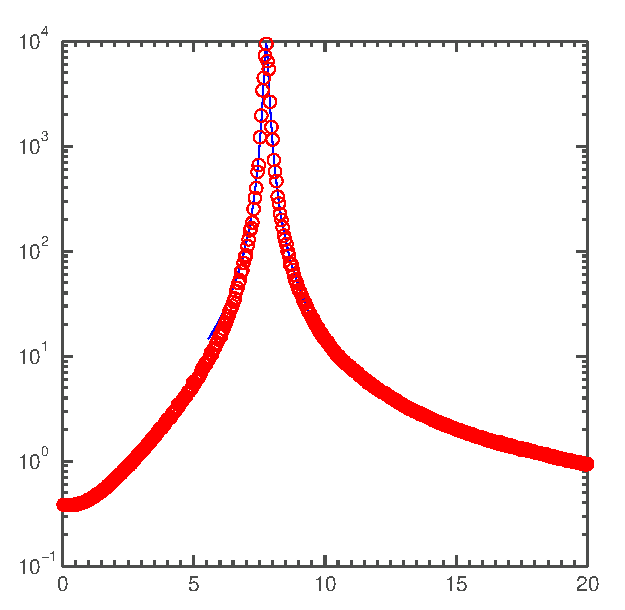
\includegraphics{/home/schuberm/Dropbox/git/plots.nogit/images/sed.eps}}
\renewcommand{\figure}{Fig.}
\caption{(Colour online) Spectral energy density plots for the selected modes along k=[1,0,0] of a 4x4 superlattice as shown in Figure~\ref{fig:dispersion}. Dark blue corresponds to a superlattice without mixing, red corresponds to mixing of 80/20 and light blue corresponds to mixing of 60/40.}
\label{fig:sed}
\end{center}
\end{figure}
%%%
\begin{figure}%[H]
\begin{center}
\scalebox{0.8}{ 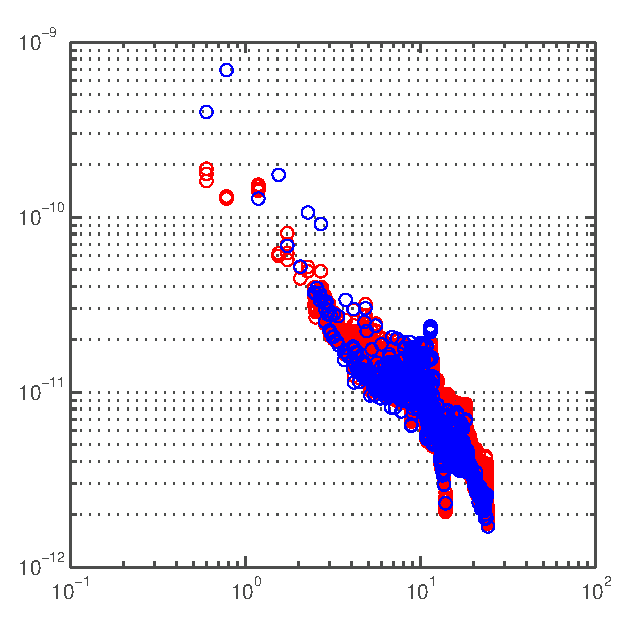
\includegraphics{/home/schuberm/Dropbox/git/plots.nogit/images/NMD_v_ALD.eps}}
\renewcommand{\figure}{Fig.}
\caption{Comparison between lifetimes from NMD and ALD in a 4x4 superlattice without interfacial mixing.}
\label{FIG:NMD_v_ALD}
\end{center}
\end{figure}

Anharmonic lattice dynamics \cite{PhysRevB.79.064301} (ALD) perturbs the harmonic solutions from HLD to obtain phonon lifetimes. ALD cannot determine the effects of mixing because of the analysis is based in reciprocal space and as such imposes the same geometric mixing to all unit cells. Hence, ALD was used to validate the lifetimes in a 4x4 superlattice without interfacial mixing. Figure~\ref{FIG:NMD_v_ALD} shows no systematic bias between ALD and NMD for shorter lifetimes, with some scatter at the longer lifetimes. In general, ALD lifetimes are expected to be larger than NMD lifetimes because ALD neglects the contribution from $n$ order phonon processes, where $n$ is greater than 3. 

Green-Kubo (GK) simulations, previously validated against the non-equilibrium direct method \cite {PhysRevB.79.075316}, were performed on the the same MD domain that was used in the NMD approach. In order to minimize the error in the GK predictions, the process outlined by Chen \cite{Chen20102392} was followed.  Uncertainty in the NMD prediction was found by varying the initial guesses for the fitting parameters and taking the standard deviation of the thermal conductivity. Uncertainty in the GK prediction was found by determining the effect of removing a single MD seed upon the average estimate. From Table~\ref{TB:validate}, the predictions for superlattices without mixing lie within the uncertainty of one another. For superlattices with mixing, NMD predicts a lower in-plane thermal conductivity, differing systematically by about 20\% while the cross-plane predictions, however lie within the uncertainty. For the remainder of this work, the 80/20 system is used to discuss the effects of mixing upon phonon properties.
%%%
\begin{table}
\begin{center}
\begin{tabular}{lcc}
\hline\noalign{\smallskip}
&\multicolumn{2}{c}{Method} \\
\cline{2-3}\noalign{\smallskip}
$k$ & NMD  & GK  \\
\noalign{\smallskip}\hline\noalign{\smallskip}
%Cross-Plane Perfect  & 0.235 $\pm$ 0.001& 0.2638 $\pm$ 0.0174\\
%Cross-Plane Mixed     & 0.169  $\pm$ 0.001   &   0.2025 $\pm$ 0.0065 \\
%In-Plane Perfect   & 0.5134 $\pm$ 0.005 & 0.5263 $\pm$ 0.0263  \\
%In-Plane Mixed   & 0.2545 $\pm$ 0.002 & 0.2974 $\pm$ 0.0052  \\
%Cross-Plane Perfect  & 0.24 $\pm$ 0.001& 0.26 $\pm$ 0.02\\
%Cross-Plane Mixed     & 0.17  $\pm$ 0.001   &   0.20 $\pm$ 0.01 \\
%In-Plane Perfect   & 0.51 $\pm$ 0.005 & 0.53 $\pm$ 0.03  \\
%In-Plane Mixed   & 0.25 $\pm$ 0.002 & 0.30 $\pm$ 0.01  \\
Cross-Plane Perfect  & 0.26 $\pm$ 0.001& 0.26 $\pm$ 0.02\\
%Cross-Plane 0.9/0.1    & 0.18  $\pm$ 0.001   &   0.21 $\pm$ 0.01 \\
%Cross-Plane 0.8/0.2    & 0.17  $\pm$ 0.001   &   0.20 $\pm$ 0.01 \\
%Cross-Plane 0.6/0.4    & 0.18  $\pm$ 0.001   &   0.17 $\pm$ 0.01 \\
Cross-Plane 0.8/0.2    & 0.17  $\pm$ 0.001   &   0.18 $\pm$ 0.01 \\
Cross-Plane 0.6/0.4    & 0.18  $\pm$ 0.001   &   0.19 $\pm$ 0.01 \\
In-Plane Perfect   & 0.54 $\pm$ 0.005 & 0.53 $\pm$ 0.03  \\
%In-Plane 0.9/0.1   & 0.32 $\pm$ 0.002 & 0.37 $\pm$ 0.01  \\
In-Plane 0.8/0.2  & 0.25 $\pm$ 0.002 & 0.30 $\pm$ 0.01  \\
In-Plane 0.6/0.4   & 0.20 $\pm$ 0.002 & 0.26 $\pm$ 0.01  \\
\noalign{\smallskip}\hline
\end{tabular}
\end{center}
\renewcommand{\table}{Table.}
\caption{A comparison of the thermal conductivity predictions [$Wm^{-1}K^{-1}$] predictions for a 4x4 superlattice.}
\label{TB:validate}
\end{table}
%%%
%%%
\renewcommand{\textfraction}{0.0}
\begin{figure}%[H]
\begin{center}
\scalebox{1}{ \includegraphics{/home/schuberm/Dropbox/git/plots.nogit/images/lifvomega.eps}}
\renewcommand{\figure}{Fig.}
\caption{Lifetimes for perfect and mixed systems. From top to bottom 2x2, 4x4, 8x8 and 14x14 superlattices. The black line corresponds to the Ioffe-Regel criterion, $2\pi\omega^{-1}$. The brown line corresponds to a $A_2\omega^{-2}$ fit. The green line corresponds to a $A_4\omega^{-4}$ fit.}
\label{FIG:lifetime}
\end{center}
\end{figure}
%%%
%%%
\begin{figure}%[H]
\begin{center}
\scalebox{1}{ \includegraphics{/home/schuberm/Dropbox/git/plots.nogit/images/MFP_cp.eps}}
\renewcommand{\figure}{Fig.}
\caption{Phonon mean free path normalized by the period length contribution to the cross-plane thermal conductivity. From top to bottom 2x2, 4x4, 8x8 and 14x14 superlattices. Lines are used to guide the eye.}
\label{FIG:MFP_cp}
\end{center}
\end{figure}
%%%
As interspecies mixing is introduced, there is a downwards shift in phonon lifetimes, particularly for the higher frequency modes as seen in Figure ~\ref{FIG:lifetime}. A Rayleigh scattering scaling ($\omega^{-4}$) is observed at larger frequencies for smaller period lengths (2x2, 4x4). However, because the determination of $\tau\kv$ does not distinguish between phonon scattering mechanisms, the $\omega^{-4}$ scaling diverges at low frequencies and is replaced by $\omega^{-2}$ scaling. For the larger period length superlattices (8x8, 14x14), the non-mixed systems have two $\omega^{-4}$ scalings, which disappear as mixing is introduced. Interspecies mixing strongly effects lifetimes in short period superlattices, shifting some modes below the Ioffe-Regel criterion. As the modes for a given superlattice have a plane wave structure, reaching the Ioffe-Regel criterion is an indication of not spatial localization but rather temporal localization.

A computational limitation of NMD is the challenge in resolving longer wavelength modes because of the limited resolution of the Brillouin zone enforced by the MD domain. This effect is observed in Figure~\ref{FIG:MFP_cp}, where the finite number of resolved wavevectors leads to what would appear as noise in the contribution distribution at longer MFPs. Although size-independent thermal conductivity was achieved, careful analysis of these longer wavelength modes would be beneficial. This has been observed in other mode by mode techniques, such as the real space force constant extraction method used by Esfarjani \cite{PhysRevB.84.085204}, where resolving modes at the zone center presents remains an open question.

Although the thermal conductivity predictions from NMD and GK for systems without interfacial mixing agree, mixing introduces discrepancies that cannot be explained by statistical uncertainty (Table~\ref{TB:validate}). The original assumption of using eigenvectors obtained from unperturbed unit cells to map atomic velocities to the normal deserves to be reexamined. The modified superlattice dispersion allows one to capture the effects of the secondary periodicity upon group velocities and lifetimes. However, interfacial mixing disrupts this secondary periodicity and thus alters the dispersion. As such, although some modes continue to exist in the mixed systems, others are effectively destroyed. This is observed in the SED of select modes as seen in Figure~\ref{fig:sed}, where some peaks continue to be pronounced, indicative that this modes exists, while others diverge from the perfect case and begin to pick up frequencies associated with other modes that are captured in the NMD.  In other words, the superlattice phonons which emerge from the secondary periodicity are effectively destroyed by the interfacial mixing. 

From Figure~\ref{FIG:MFP_cp}, there is a clear reduction in the contribution to cross-plane thermal conductivity of modes with a MFP greater than the period length as period length increases. This is consistent with the theoretical predictions from Mahan that a transition from a wave-regime to particle-regime will occur \cite{PhysRevLett.84.927,PhysRevB.56.10754}. This trend is not observed in the contribution curves for the in-plane conductivity, where the peak MFP remains unchanged as a function of period length. For short period superlattices, interfacial mixing shifts in the peak MFP towards shorter lengths and reduces its respective contribution. For mixed 2x2, 4x4 and 8x8, the peak MFP is shifted arbitrarily close to the period length, indicative of the transition of thermal transport from superlattice phonons to thermal transport from phonons of MFP on the order of the period length. This trend further supports the point of superlattice phonons being destroyed by mixing, and thus diminishing the wave effects of the secondary periodicity upon cross-plane thermal conductivity. At large enough period lengths, the effect of interspecies diffusion has a negligible effect on phonon MFP, as the lifetimes become less effected with increasing period length (Figure~\ref{FIG:lifetime}). 

\section{Superlattice phonons}

In previous experimental work \cite{PhysRevLett.73.740,PhysRevB.75.195309}, the coherent phonons fell into different classes: Brillouin oscillations, impulse stimulated Raman scattering and coherent acoustic Bragg reflection. The latter can be observed in a pump-probe setup where modes that satisfy the Bragg reflection criterion for constructive interference
\begin{equation}\label{EQ:Coh}
2D \cos \theta = m \lambda,
\end{equation}
where $D$ is the superlattice period length, $m$ is an integer and $\theta$ is the angle of incidence of phonon with wavelength $\lambda$ will be selectively filtered from the transmission spectrum \cite{PhysRevLett.43.2012}.

Coherent phonon effects upon thermal transport are claimed to exist in such structures as porous silicon \cite{doi:10.1021/nl102918q} and superlattices \cite{PhysRevB.67.195311} where the artificial periodicity (from the periodicity of the pores or the alternating layers of dissimilar materials) introduces new phonon dynamics, leading to much confusion in the terminology. An attempt is made here to clarify the distinction between \textit {coherent phonon effects} and \textit{coherent phonons}.

The length scales of interest in sub-continuum thermal transport are wavelength, coherence length and mean free path (MFP). The phonon-phonon MFP, in the phonon particle picture, is typically defined as the distance travelled between particle collisions \cite{ziman_electrons_2001}. Coherence length is the distance a plane wave travels until the phase becomes uncorrelated and thus only applies in the wave picture of phonon transport. Phase is assumed to be randomized through inelastic phonon-phonon, but not elastic boundary or impurity scattering \cite{chen2005nanoscale}. However, other definitions argue that roughness and disorder, in general, destroy coherent effects \cite{PhysRevB.67.195311,dames:682}.

For thermal conductivity predictions, modes that do not propagate, do not contribute directly to the thermal conductivity. Thus, for the purposes of heat conduction in artificially periodic structures, we are not concerned with the former definition of coherent phonons (e.i.: those that satisfy the Bragg reflection criterion), but rather the coherence length of phonons. 

Chen implicitly defines phonon coherence length as proportional to the inverse of the bandwidth and notes the that MFP is, in most cases not equivalent to coherence lengths \cite {Chen_particularities,chen2005nanoscale}. Chen further argues that a phonon coherence length is not applicable to superlattices, unless the correct dispersion is used and the analysis is wave-based\cite{chen:945}, but justifies equating the MFP to the coherence length if is assumed that a scattering process randomizes phase \cite{PhysRevB.67.195311}. A review of the literature reveals no explicit form for the phonon coherence length, only heuristic analogies to the coherence lengths of electrons and photons. In classical electromagnetism, coherence length is defined as

\begin{equation}\label{EQ:Coh2}
\begin{split}
l &= \frac{c}{n\Delta \omega} 
\end{split}
\end{equation}

where c is the speed of light, $n$ is the refractive index and $\Delta \omega$ is the bandwidth. If we follow this analogy, phonon coherence length will depend upon phase velocity and bandwidth. This would produce orders of magnitude larger lengths than the corresponding bulk MFPs, and is thus not the quantity of interest.

%In the ballistic regime, do the MFP and coherence length converge? Is there some regime in which the MFP and coherence are equivalent? Here we show that the NMD approach can predict MFP, and following from the definition and analogies, can be set to the coherence length.

%The effects of coherence emerge from the stop bands that exist as a result of Brillouin zone folding as can be seen in Figure ~\ref{fig:dispersion}. 

Here we develop a wave-based approach to phonon transport in superlattices by using a unit cell that spans one period to generate the modified dispersion relation which allows one to ignore the difference between the MFP and coherence length.

\section{Summary}

To summarize, we show the reduction in the contribution to cross thermal conductivity from MFP greater than the superlattice period as the period length is increased. Differences between in-plane and cross-plane components of group velocity are responsible for the respective differences between thermal conductivity. Phonon lifetimes in superlattices can be significantly reduced by interspecies mixing, as the secondary periodicity is disrupted, thus reducing in-plane and cross-plane thermal conductivity. 

\newpage
%\bibliographystyle{apsrev}
\bibliography{superlattice.bib}

\end{document}

